\subsection{Definition}
This example deals with an aquifer which is subject to a constant recharge line source. The channel is assumed to be independent of the groundwater head and not affected by the water loss or the exchange flux. Therefore, the source term represents a steady and uniform channel located above the aquifer. The cross-section of the channel is rectangular (Fig.~\ref{river_groundwater}). 

\begin{figure} [htb!]
 \centering
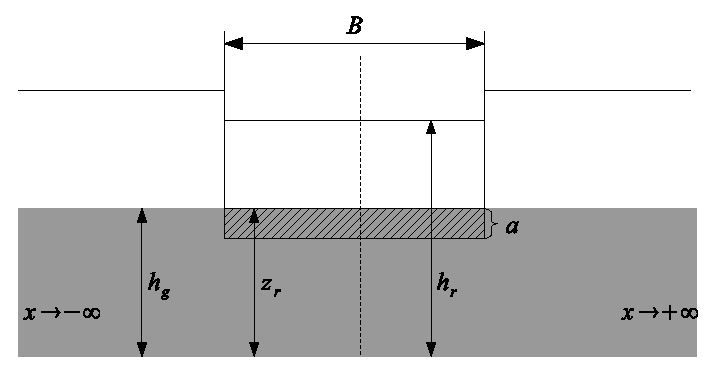
\includegraphics[width=0.6\columnwidth] {Chapter5/figure/river_groundwater.eps}
\caption{The illustration of the cross section of the channel/groundwater.}
 \label{river_groundwater}
\end{figure}

The integrated recharge flow that provides the link between the channel and the groundwater is defined by Eq.~\ref{eq:GW_riverSource} \cite{Gunduz2005216}.

\begin{eqnarray}
q^{ex} =  \left\{
  \begin{array}{l l}
    -K_{\Lambda}{P}\frac{(h_r - h_g)}{a} & \quad \text{$h_g>(z_r-a)$}\\
    \\
    -K_{\Lambda}{P}\frac{(h_r - (z_r-a))}{a} & \quad \text{$h_g\leq(z_r-a)$}\\
  \end{array} \right. 
\label{eq:GW_riverSource}
\end{eqnarray}
%
where $K_{\Lambda}$ is the channel bed conductivity, $B$ is the channel width, $a$ is the channel bed thickness, and $h_r$ is the channel flow head, $h_g$ is the groundwater table. The wetted perimeter $P= 2 (h_r-z_r) + B$ for rectangular channel where $z_r$ is the height of the top of the channel bed.

In this benchmark, the aquifer size is 20~m$\times$ 10~m with the source term at the left boundary (See Fig.~\ref{channel_location}). The initial groundwater head is 0~m. The channel source term is the boundary condition at one side, at the opposite boundary the head is fixed with 0~m. At the remaining boundaries no-flow is imposed.

For the spatial discretization either $24\times 12$ quadrants or hexahedra are used as well prisms which are generated by cutting the hexahedra into two parts. The hexahedra or prism height is 1~m. The time step is 1 minute.
Simulation parameters for the aquifer and the channel source term are given in Table.~\ref{GW_ChannelPercolation1}.
%
\begin{table}[H]
 \centering
 \caption{Parameters for channel source term examples.}
 \centering \label{GW_ChannelPercolation1}
\begin{tabular*}{0.9\textwidth}{@{\extracolsep{\fill}}llrr}
\hline\noalign{\smallskip}
Symbol& Parameter & Value & Unit\\ 
\hline\noalign{\smallskip}
\multicolumn{4}{c}{\bf Aquifer}		\\  
\hline\noalign{\smallskip}                             
		$S$ 	 	& 	  Storage 					             & $0.2$ & $-$ \\               
		$\mu$ 		& 	  Viscosity  				           & $1.0\times 10^{-3}$ & $Pa\cdot$\\ 
		$K$ 	 	& 	  Conductivity 				         & $1.0\times 10^{-3}$ & $m/s$ \\   
		$L$ 	 	& 	  Thickness 				            & $25$ & $m$ \\ 
\hline\noalign{\smallskip}          
\multicolumn{4}{c}{\bf Channel source term}				 	\\       
\hline\noalign{\smallskip}                             
		$h_r$ 		& 	  Channel water surface 	   & $3$ & $m$ \\                       
		$z_r$ 		& 	  Bed top location			       & $0$ & $m$ \\                       
		$a$ 	 	& 	  Bottom sediment thickness & $0.3$ & $m$ \\                     
		$B$ 	 	& 	  Channel width 			         & $34$ & $m$ \\                    
		$K_{\Lambda}$	 		& Bed conductivity 	  & $1.0\times 10^{-6}$ & $m/s$ \\
 \noalign{\smallskip}\hline
 \end{tabular*}
\end{table}
%
A constant recharge value of 4.0$ \times 10^{-4} m^2/s$ is obtained from Eq.~\ref{eq:GW_riverSource} when the properties
of the channel are defined as those values in Table.~\ref{GW_ChannelPercolation1}. Because this problem is
symmetric for uniform and isotropic conditions in the aquifer and only half of the domain
is taken into account. Therefore, the constant Neuman boundary condition is assigned with the half of
the recharge value (2.0$\times 10^{-4} m^2/s$).

\subsection{Solution}

R. E. Glover \cite{Glover:74} presented an analytical solution for a constant line source in an infinite aquifer domain in 1978, which gives the groundwater head at any point of the source line by the following equation,
%
\begin{eqnarray}
h = q^{ex}\sqrt{ \frac{\mu t}{\pi \rho g \kappa L S_y}} 
\label{GW_Glover}
\end{eqnarray}
%
where $q^{ex}$ is the recharge rate [L$^2$/T], $L$ is the saturated thickness of the aquifer [L], $\kappa$ is the permeability of the aquifer [L$^2$/T], $S_y$ is the specific yield of the aquifer [-], $t$ is the time [T].

\subsection{Results}

Comparison of simulation results and analytical solution is given in Fig.~\ref{GW_Results_ChannelPercolation_quad}
for quadrants and in Fig.~\ref{GW_Results_ChannelPercolation_hex} for hexahedra.
%
\begin{figure} [htb!]
 \centering
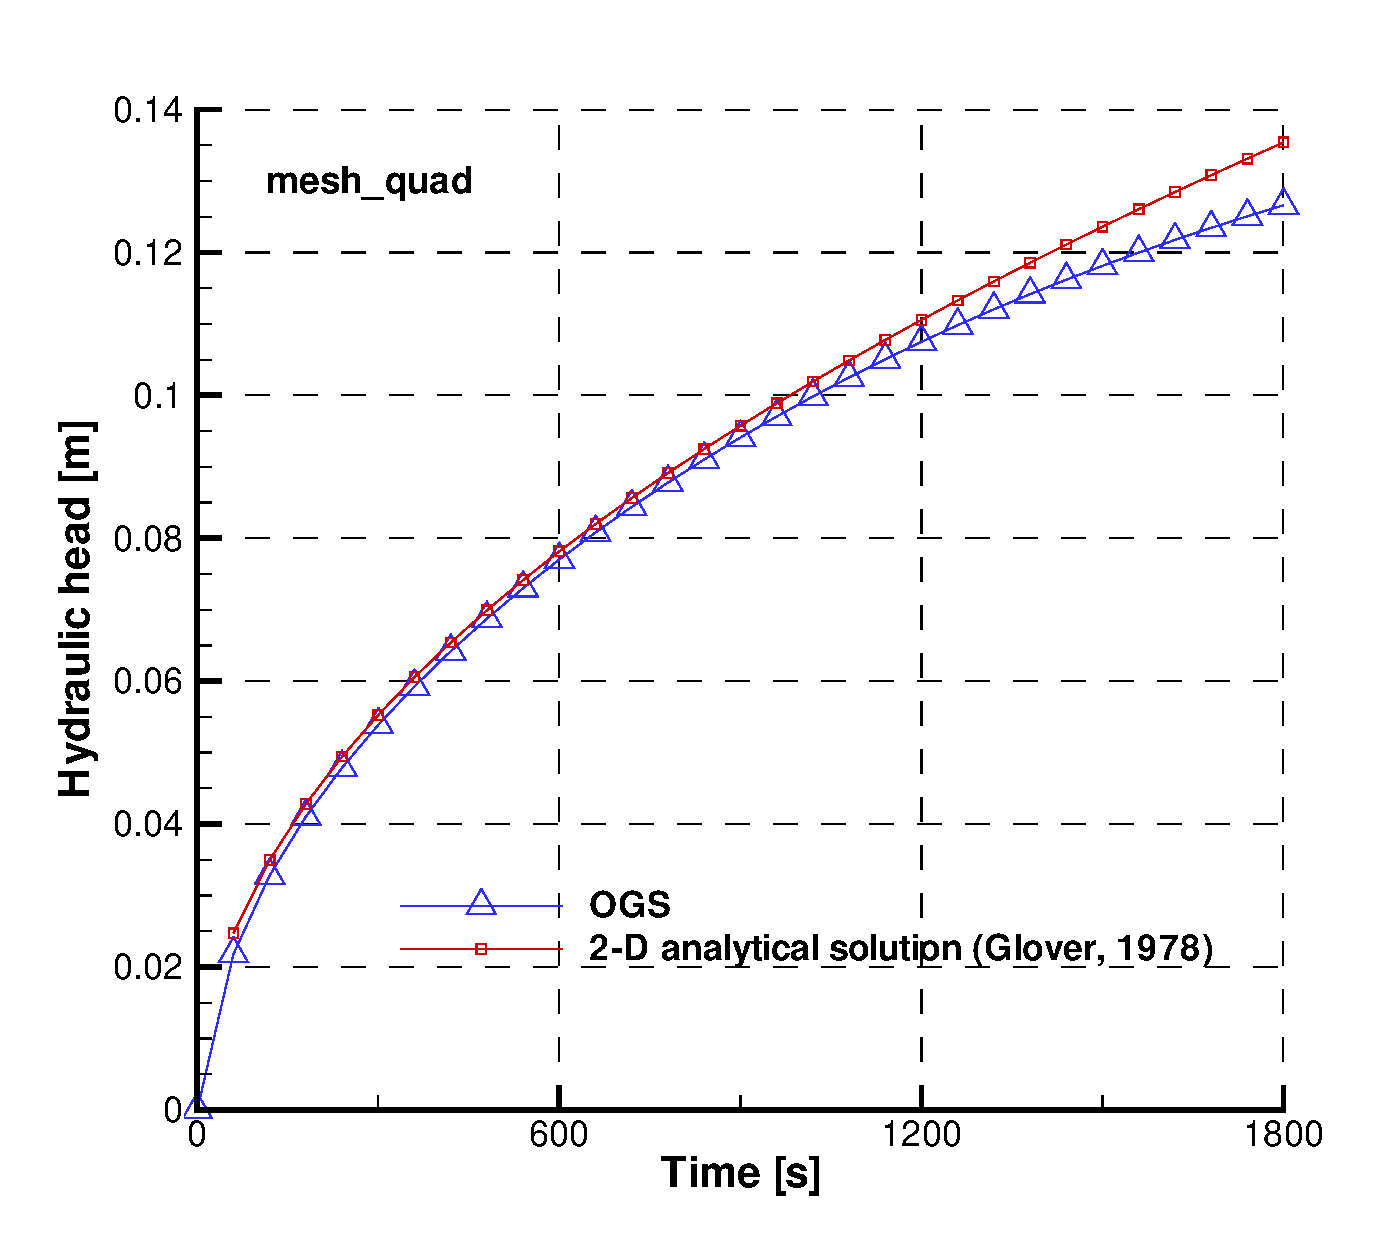
\includegraphics[width=0.6\columnwidth] {Chapter5/figure/riv1_quad_point.eps}
\caption{Results with quadratic elements and analytical solution for confined aquifer below uniform and steady channel.}
 \label{GW_Results_ChannelPercolation_quad}
\end{figure}
%
\begin{figure} [htb!]
 \centering
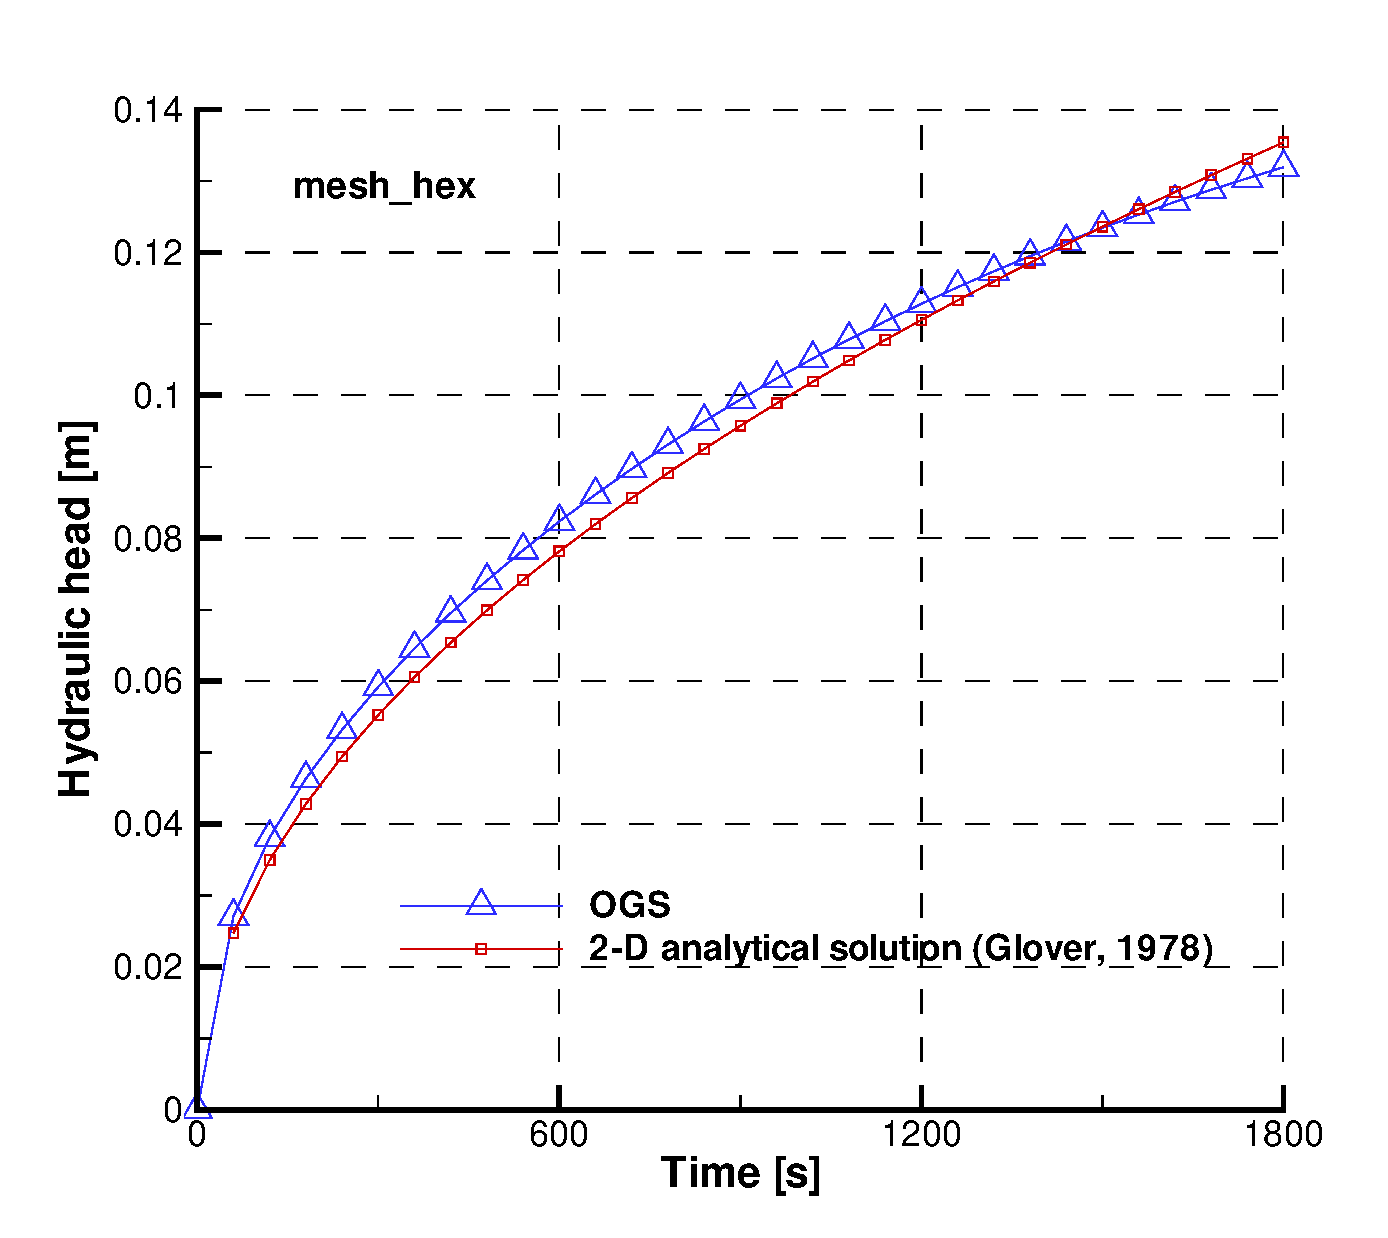
\includegraphics[width=0.6\columnwidth] {Chapter5/figure/riv1_hex_point.eps}
\caption{Results with hexahedral elements compared with the analytical solution for confined aquifer below uniform and steady channel.}
 \label{GW_Results_ChannelPercolation_hex}
\end{figure}

The small differences between Fig.~\ref{GW_Results_ChannelPercolation_quad} and Fig.~\ref{GW_Results_ChannelPercolation_hex} are mainly caused by the channel source term. In the model with hexahedral elements, the channel source term is defined as a line source at the left-top boundary of the domain (Fig. \ref{channel_location}). 

\begin{figure} [htb!]
 \centering
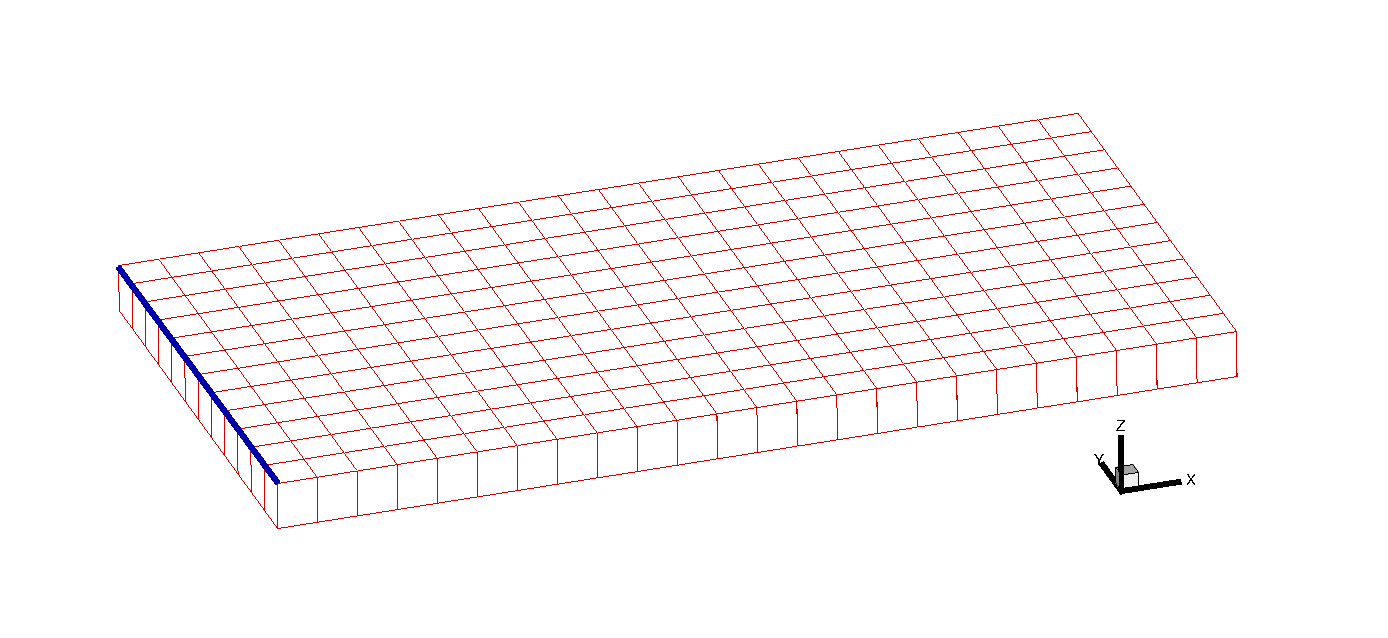
\includegraphics[width=0.8\columnwidth] {Chapter5/figure/channel_location.eps}
\caption{Computational domain and source term location.}
 \label{channel_location}
\end{figure}
